%!TEX root = ../these.tex

\section{Технологические ограничения}
\label{sec:cut.PC}

Полученный любым способом маршрут движения режущего инструмента~
\eqref{eq:cut.tuple},
должен быть исполнен на конкретном промышленном оборудовании ---
режущей машине с ЧПУ.
Это накладывает ряд существенных ограничений на решение задачи резки,
в терминах формулы \eqref{eq:cut.problem} ---
существенно ограничивает проблемное пространство
$\mathfrak G$.
Рассмотрим некоторые из этих ограничений.

\subsection{Позиции точек врезки и выключения инструмента}

Это естественно возникающие технологические ограничения,
которые естественно называть <<геометрическими>>,
вызваны тем,
что, как сказано выше,
точка врезки должна располагаться на некотором
ненулевом расстоянии от контура детали.
Кроме того, они не должны попадать внутрь других деталей,
с учетом припуска на ширину реза.
Конкретные расстояния определяются используемыми технологиями.

Введем обозначения:
эквидистанты замкнутых контуров
$C_1, C_2, \dots C_N$,
удаленные от них на расстояние $d$,
обозначим за
$C_1^{+d}, C_2^{+d}, \dots C_N^{+d}$,
а ограниченные этими эквидистантами
двумерные геометрические объекты ---
$\widetilde C_1^{+d}, \widetilde C_2^{+d}, \dots \widetilde C_N^{+d}$,
$\widetilde C_i^{+d} \in \mathbb R \times \mathbb R$.
Для внешних контуров берется внешняя эквидистанта,
для внутренних --- соответственно внутренняя.
Далее, пусть
$OUT = \{i_1^+, i_2^+, \dots i_{N^+}^+\} \subseteq \overline{1, N}$ ---
множество индексов внешних контуров,
а
$IN = \{i_1^-, i_2^-, \dots i_{N^-}^-\} \subset \overline{1, N}$ ---
множество индексов внутренних,
$|OUT|=N^+$,
$|IN|=N^-$,
если внутренних контуров на раскройной карте нет,
то $N^+=N$, $N^-=0$, $IN=\varnothing$.

Если минимальное расстояние от контура детали до точки врезки
$d_1$,
то позиции точек врезки должны удовлетворять условию
$M_i \in G_M, \forall i \in \overline{1, N}$,
где
$$
G_M = \left(\mathcal B \setminus \bigcup_{i \in OUT} \widetilde C_i^{+d_1} \right)
  \cup \bigcup_{i \in IN} \widetilde C_i^{+d_1}
$$

Аналогично может быть записано ограничение для
позиций точек выключения инструмента
$M^*_i \in G_{M^*}, \forall i \in \overline{1, N}$:
$$
G_{M^*} = \left(\mathcal B \setminus \bigcup_{i \in OUT} \widetilde C_i^{+d_2} \right)
  \cup \bigcup_{i \in IN} \widetilde C_i^{+d_2}
  ,
$$
где
$d_2$ --- допустимое расстояние
от контуров деталей до точек выключения инструмента;
как правило
$0 \leqslant d_2 < d_1$.

\begin{figure}
  \centering
  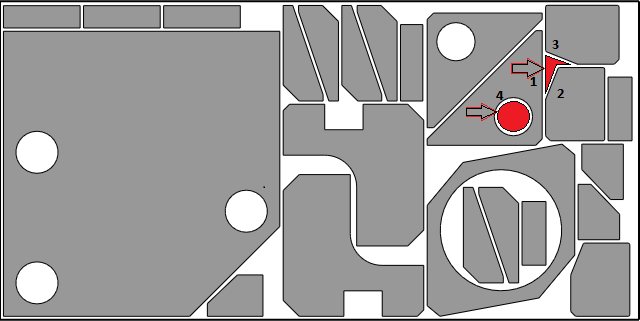
\includegraphics[width=0.9\textwidth]{pierce-area.png}
  \caption{
    Пример двух геометрических областей на раскройной карте,
    допустимых для задания точек врезки
  }
  \label{fig:cut.pierce-area}
\end{figure}

На рис.~\ref{fig:cut.pierce-area}
показаны стрелками и выделены цветом
две геометрические области листа,
одна, определяемая
внешними граничными контурами деталей,
обозначенных цифрами
\textit{1, 2} и \textit{3},
и вторая ---
внутренним граничным контуром
\textit{4}.
Минимально допустимое расстояние
от граничных контуров
\textit{1--4} до возможных точек врезки
$d_1=9.5$~мм.
